\documentclass[a4paper]{article}

\usepackage[english]{babel}
\usepackage[utf8x]{inputenc}
\usepackage{amsmath}
\usepackage{graphicx}
\usepackage[colorinlistoftodos]{todonotes}

\title{Preliminary Thesis Results}


\begin{document}
\maketitle

\begin{abstract}
I've completed over 20\% of the proposed experiments in my thesis experimental protocol, yielding over 20,583 data points on which to do preliminary analysis. I have early results for three species distribution modeling methods on four training set sizes, four different spatial resolutions, and 44 different computing configurations. Preliminary data analysis show little to no correlation between computing configuration variables (vCPU and RAM) and model execution time.   The only clear relationship I've uncovered is the strong positive relationship between the number of training examples used to fit the model and the execution time.  Two predictive models for execution time, a linear model with multiple predictors, and a boosted regression tree model, were developed to estimate running time of future SDM scenarios.  The question now is whether to be patient and run the remaining (and more expensive) experiments, or refine the experimental protocol to one that responds better to the computer hardware variables.
\end{abstract}

\section{Methods}

\subsection{Experimental Variables}
\subsubsection{CPU Cores}
Virtual CPU cores (vCPU) are included as an experimental variable, because their addition to a problem is the only way to to directly increase the number of instructions being executed by the machine.  With a single processor machine, instructions must be sequentially executed.  If there are multiple processes running on a machine at one time, the instructions must be interleaved to give the illusion of simultaneous execution.  If one or more cores are added, the workload can be split across these processors to execute the instructions in parallel.  If a modeling algorithm is a serial algorithm (most SDMs are), adding multiple cores can improve its speed by offloading system processes and other work to other processors, leaving one processor for model execution.  If the model is designed for parallel execution, adding cores can speed up the execution of the algorithm proportionally to the percentage of the program that can execute in parallel (Amdhal's Law).  Most programs require at least a small amount of serial code (to synchronize results or initialize runs), so infinite speedup is not possible.  The algorithm I'm using (boosted regression trees in the gbm R package) is designed with a small portion of parallel code, so should demonstrate at least a small speedup  with the addition of multiple processor cores.

\subsubsection{Memory}
Adding virtual memory (RAM) to a process can increase its execution time by reducing the number of times the computer must retrieve data from the physical storage device (e.g., the hard disk).  Operating on data from the hard disk, especially a traditional mechanical one) is orders of magnitude slower than operating on instructions that are already stored in the computer's main memory. If the size of the data to be executed on exceeds the size of the RAM, the computer will automatically chunk it up, and go back and forth between the hard drive and main memory.  By increasing the size of the memory, we reduce the need to go to the hard disk, thus increasing execution time. 

\subsubsection{Training Examples}
All of the competitive species distribution models (generalized linear models, regression trees, adaptive splines, etc) are instances of supervised learning.  Supervised learning methods required a set of tagged training examples that show the 'correct' answer, along with that answer's input conditions.  The goal of the learning method is then to learn the function \textit{h(x)} that approximates the mapping between input conditions to answer.  More tagged examples gives the learner more data with which to work, and, in theory, should demonstrate higher accuracy.  However, giving the learner more data means that it will need to fit a more complicated response surface. I hypothesize that giving the modeling algorithm more training examples will increase the time it takes to learn \textit{h(x)}.

\subsubsection{Spatial Resolution}
The fitting of the models is essentially non-spatial: the environmental covariates are pre-extracted from the predictor layers, processed, and fed to the model.  Once the model is fit, however, the response \textit{h(x)} is projected onto the RPC8.5 scenario for AD2100.  A low spatial resolution prediction grid will have only a relatively small number of grid cells to project onto. As spatial resolution increases, the number of cells on which to project increases exponentially.  Thus, while the fitting time of the model is unlikely to be affected by the spatial resolution of the response, the time it takes to produce a gridded output will likely increase significantly at higher resolutions.

\subsection{Experimental Design}
In an ideal world, I would run carefully controlled experiments in a full factorial design for each of these experimental variables, with a suitable number of replicates per cell for robust inference.  However, there are a couple reasons this is not possible in my case.  
\begin{enumerate}
\item \textbf{Cost} It is prohibitively expensive to test every combination of the variables, particularly with replicates.  
\item \textbf{Time} I am also limited in the time I have to run these experiments, and do not have the thousands of hours needed to run all of these simulations.
\item \textbf{Platform} Cloud platform providers do not allow unconstrained creation of arbitrary machine types.
\end{enumerate}

\begin{figure}
	\centering
		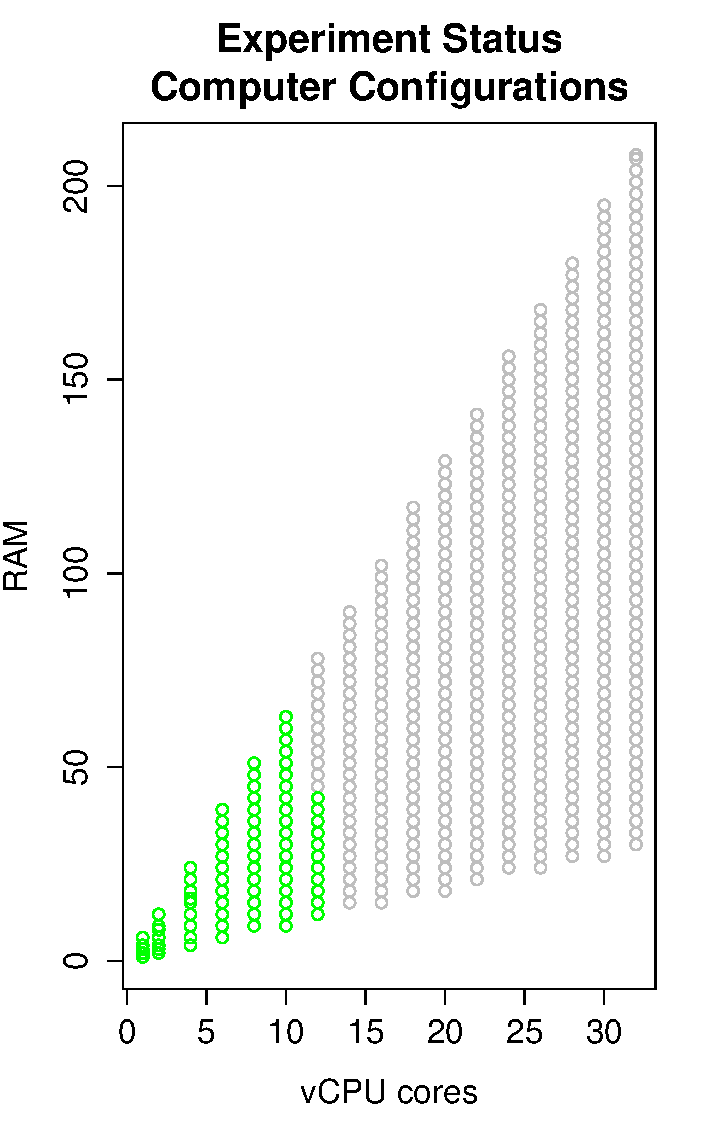
\includegraphics[width=0.6\textwidth]{config_status.png}
	\caption{Distribution of experiments across computing types.  Experiments in green have been completed to-date.}\label{fig:conf_status}
\end{figure}

Because I can't run all of the experiments, I came up with a compromise scheme that attempts to balance capturing the within-variable variance (more replicates) with the interactions between the variables (more cells) .  I do this by running one main series of experiments with a selected subset of algorithm inputs (training examples and spatial resolution) on a wide variety of computer types (vCPU and memory), and then a couple of sensitivity analyses that capture the response of the algorithm to a change in a particular input. 

\subsubsection{Main Series}
The goal of the main series is to capture the interactions within variables, and to capture the contribution of running the algorithms on increasingly more powerful machine types.  Because execution time can demonstrate non-linear and/or non-additive responses when run on alternate hardware, it's important to test as many combinations of the two computing variables as possible.  On each computer type, I have a standard set of 160 experiments to run (4 spatial resolutions x 4 training example sets x 10 replicates). All of these experiments are done on the \textit{Picea} pooled niche data set. Figure \ref{fig:conf_status} shows the computing instances that I use in the main series.

\subsubsection{Taxa Sensitivity}

\begin{table}
\centering
\begin{tabular}{l|r}
vCPU & Memory \\\hline
1 & 3 \\
2 & 8\\
3 & 15\\
8 & 30\\
16 & 60\\
32 & 208
\end{tabular}
\caption{Computing configurations in the taxa sensitivity experiments.}\label{tab:tSensitivity}
\end{table}

There is not a clear reason why the execution times should vary between different taxa, because the model will fit with the same number of training examples and project onto the same spatial grid.  But, to evaluate whether differences among taxa do occur, and if so, to the magnitude of the variation, I have a series of experiments that test on four different taxa.  These taxa are \textit{Picea}, \textit{Tsuga}, \textit{Quercus}, and \textit{Betula}.  The tSensitivty set is run on 6 instance types, as shown in Table \ref{tab:tSensitivity}.

\subsubsection{Training Example Sensitivity}

\begin{figure}
\centering
\includegraphics[width=0.5\textwidth]{tSensitivity.png}
\caption{\label{fig:tSensitivty}Number of training examples included in the  training example sensitivity set of experiments.}
\end{figure}

To test the affect of adding training examples on the fitting time of the algorithm, I have a set of measurements to evaluate this effect on a single computing type for more examples than I have in the main series of experiments.  Different numbers of training examples between 100 and 30,000 are examined, as shown in Figure \ref{fig:tSensitivty}.

\subsubsection{Spatial Resolution Sensitivity}
To evaluate the hypothesis of an exponential increase in model projection time with a proportional decrease in spatial resolution of the output grid, I have planned a sensitivity test for spatial resolution.  Fitting a standard model, I will evaluate the projection time at between 0.1 and 1 degrees resolution by 0.1 degree step size.


\subsection{Platform}
I am using the Google cloud platform (a.k.a Google Compute Engine) to complete all of my experiments.  On this platform, Google rents out isolated portions (e.g., instances or nodes) of its massive computing infrastructure to consumers. The consumers, like me, pay per minute for the resources that they use.  These nodes can be very basic (1 vCPU and 0.6 GB RAM) or exceptionally powerful (32 vCPU and 208GB RAM), or nearly anywhere in between. Along with the platform, Google has developed a set of APIs for automated control of the virtual computing instances, as well as a GUI console for interactive control.

The main reason for this choice is the ability to create 'custom' instance types.  Other notable cloud providers (e.g., Amazon Web Services) provide a large number of predefined instance types, some even more powerful than Google's top-end, but do not allow you to create an instance with an arbitrary number of vCPU cores and memory.  Google allows you to do this, which fits well into my experimental framework.

\begin{figure}
\includegraphics[width=1.1\textwidth]{file-page1.jpg}
\caption{A flowchart describing the way in which virtual infrastructure is managed to run SDM simulations.}\label{fig:flowchart}
\end{figure}

My setup draws on a bit on the design of larger systems like Hadoop, which create frameworks for massively large and distributed fault-tolerant systems. In short, I have one Master Node that hosts a database and a control script, and a pool of compute nodes that are fault-tolerant and designed only for computing. The compute nodes don?t have to know anything about the progress of the entire project and can handle being shut down mid-run, and the control node doesn?t have to know anything about the simulations being computed.  At any one time I will have one or many servers that will actually be doing the job of computing the species distribution models and assessing their time and accuracy (compute nodes). At the same time, I will have one server that hosts the database and the API, starts and stops the computing instances, and cleans up the workspace when necessary (Master Node). This approach allows me to use Google's preemptible instances, which cost much less, but have the potential to be dropped due to system demand at any time. Figure \ref{fig:flowchart} shows a conceptual diagram of the platform logic.

\subsubsection{Configuring and building virtual instances}
The steps to building and configuring the pool of computing nodes takes follows this general process: 
\begin{enumerate}
\item The MasterNode.py script uses the (daemonized [always running]) node.js web backend to query the database to ask 'What experiments have not yet been marked as DONE?'. The computing script could also mark experiments as "LEGACY", "INTERRUPTED", or "ERROR" depending on the conditions at runtime. If they have not yet been computed, they are marked in the database as "NOT STARTED". So MasterNode asks for everything that?s not "DONE", and forces a re-compute if a simulation errored or was cut short.
\item The central database, via the API, responds with a JSON object that contains the number of cores and memory needed for the next experiment (but not the other experimental parameters like number of training examples or spatial resolution).
\item MasterNode parses the JSON and then uses the gcloud tools to create a pool of computers that have the memory and number of cores specified by the database response. This pool of virtual instances is automatically created with a startup script that installs the necessary software and files to run the computing experiments.
\end{enumerate}
\subsubsection{Running the simulations and reporting the results}
Now that I have the pool of virtual instances at my disposal, I can use them to run the SDM simulations, time their execution, and report back to the central database. There are typically between 160 and 400 simulations to be done for every computing configuration, so on each node is an inner loop that looks like this:
\begin{enumerate}
\item Startup script installs git, mysql, and R. Git clones the most recent version of the project repository which has all of the files needed for the computation. R starts execution of the timeSDM.R script which controls the flow of execution for this node.
\item RScript queries the central database to ask 'I am a compute of x cores and y GB memory, what experiments can I do?'.
\item The database responds with a single JSON row that contains all of the necessary parameters to actually run the SDM simulation (spatial resolution, taxon, number of training examples, etc).
\item RSCript parses the database response and loads the correct set of variables, then runs the SDM model.
\item RScript reports results back to the database and marks that experiment as "DONE".
\item Repeat until no experiments that are not "DONE" remain to be completed by a computer of this number cores and amount of memory.
\end{enumerate}

If an instance gets shut down due to preemption (or my incompetence) a shutdown script will be fired. This script records in the database that the experiment was cut off (INTERRUPTED) at some point before successful completion, and that it should be completed again in the future.

\subsubsection{Managing virtual infrastructure}
Because Google charges you by the minute as you use their servers, and because I have to do a lot of different experiments and don?t have that much time do them, it is ideal to automatically tear down the servers and start a new pool as soon as one computing configuration has finished. So, while the computing nodes are doing their computing thing, the MasterNode repeatedly polls the central database to determine the current position within the experiment grid.
\begin{enumerate}
\item MasterNode uses the API to ask the database 'What percentage of the experiments in this group have been completed?'
\item The database responds with a percentage ("DONE" / total).
\item If the percentage is 100 (all experiments have been completed within the current configuration setup):
\begin{enumerate}
\item MasterNode will use gcloud to delete the individual server instances, the instance group pool the they are part of, and the template used to create the instances. After this, only the Master Compute Node server with the database on it still remains in my pool of Google resources. 
\item Repeat.  Configure and build a new pool of instances for the next memory/cores combination.
\end{enumerate}
\item Otherwise, continue polling.
\end{enumerate}

\subsection{Modeling Protocol }
\subsubsection{Data Origin \& Preparation}
The taxon occurrence data is from the Neotoma Paleoecological Database.  All records for the given taxon were downloaded from Neotoma, using the API.  A python script was used to identify all of the sites with that taxon.  For each site, the entire dataset was then downloaded, and the values for the taxon extracted.  The age, latitude, longitude, site identification information, and the relative abundance was stored for each Neotoma occurrence as a comma separated value file.

For each occurrence record from Neotoma for my chosen species, I extracted the bioclimatic variables at the given latitude, longitude, and years BP. The extraction was done using a python script, and the results were then stored as CSV files.

The paleo climatic predictor layers are downscaled North American CCSM 3 model simulations (Lorenz et al 2016).  The model data was obtained in netCDF format, and manipulated in python.  Bioclimatic variables were calculated from these native layers using the O'Donnell (2012) methodology, using the biovars function from the dismo R code package.  These layers have a native resolution of 0.5 degrees.

The future climatic layers, describing AD2100, for use as output predictors, were obtained from the CMIP project, HadCM3 climate model.  These layers model describe the model under the UN IPCC RCP 8.5 forcing scenario.  The layers were used to calculate bioclimatic variables, and were then resampled to various resolutions to facilitate their use as output layers in different experiments.

\subsubsection{Modeling Methodology}
I have worked with three SDM algorithms that have shown competitive accuracy results in the literature: (1) multivariate adaptive regression splines (MARS), (2) gradient boosted regression trees (GBM-BRT), and (3) generalized additive models.  All of the models were fit using the R statistical environment with standard packages for these learning methods.
The input data is communicated by the central database to the computing node, and then passed to the gbm function.  The learning parameters of the function are held constant over all experiments.  There is no database I/O inside of the function, so results should not be slow-biased by network connection or context switching.  

The experiment parameters are first communicated from the database to the computing machine.  The computing node parses the database's response and starts a new experiment session.  The correct set of training examples is loaded from disk.  It is then randomly partitioned into a testing set of $\mathcal{N}$ random training examples and ~10,000 (20\% of total) testing examples that are excluded from the training set.  Examples are converted to binary presence absence values using the Nieto-Lugilde et al (2015) method for determining local presence from fossil pollen records.  The training set is sent to the learning function where an SDM model is fit.  All models are fit on the five least correlated bioclimatic variables (bio2, bio7, bio8, bio15, bio19). The model is then projected onto the future predictor set.  The gridded output is then used to evaluate the accuracy of the model, using the testing set. Results of timing the total time, model fitting time, prediction time, and accuracy calculation time, as well as various measures of accuracy are then communicated back to the central database. 

\section{Status}

\begin{figure}
\centering
\includegraphics[width=0.5\textwidth]{CompletionByType.png}
\caption{\label{fig:experimentByCategory}Percentage of experimental variables that have been 'seen' by the SDM simulations.}
\end{figure}

\begin{figure}
\centering
\includegraphics[width=0.6\textwidth]{experimentByCategory.png}
\caption{\label{fig:completionByCategory}Percentage of experiment statuses currently in the database. }
\end{figure}

As of July 1, I've run 20,583 of the experiments as described above, which equates to approximately 20\% of the total.  Some of the models have been returning NULL, particularly at lower numbers of training examples.  I suspect that the model does not have sufficient information to fit the model with such few data points, and this has resulted in a sizable number of errors in the results set.  Figure \ref{fig:completionByCategory} shows the relative distribution of successful runs, errors, and runs yet to be started.  

While my model has 'seen' relatively few of the more powerful computing configurations, it has been exposed to all of the training examples and spatial resolutions in my protocol, so I can be fairly sure of the affect of altering these variables. Figure \ref{fig:experimentByCategory} shows the percentage of discrete values completed for each experimental variable.  I am fairly certain of the effect of spatial resolution and number of training examples on the execution time of the model.  While not quite as complete, I have seen a large number of different computer cores and a decent amount of RAM configurations as well.  The completion portion of the computing variables are also clearly shown in Figure \ref{fig:conf_status}.

I contend that, while a relatively small percentage of the total experiments have been completed, a sufficient number of runs have been done and a representative set of experimental variables have been seen to make claims about the validity of the these preliminary results.

\section{Results}
\subsection{Exploratory Analysis of GBM-BRT Data}

\begin{figure}
\centering
\includegraphics[width=0.75\textwidth]{all_vars.png}
\caption{Relationships between individual experimental variables and total time in seconds.} \label{fig:all_vars}
\end{figure}

Exploring the data leads to the surprising initial conclusion that neither the number of vCPU cores nor the amount of memory a computer significantly and consistently affects the speed performance of the model.  Over all experiments in the main series, the r\textsuperscript{2} correlation coefficients are 0.001 and 0.042 for vCPU and memory, respectively.  While these predictors do very little to influence the response, the number of training examples used to fit the model appears to be a very important factor in the total running time of the model (r\textsuperscript{2} = 0.85).  Spatial resolution shows a moderate negative correlation with time (r\textsuperscript{2} = -0.26).  Figure \ref{fig:all_vars} shows the relationships between the experimental variables and model execution time, clearly showing the strong influence of the algorithm inputs, and lack of influence of the hardware variables.

\begin{figure}
\centering
\includegraphics[width=0.65\textwidth]{Cores_and_memory.png}
\caption{Effect on time of adding additional vCPU cores.  Series are memory amounts. Evaluated by taking the median time of each combination of cores and memory.}\label{fig:cores_vs_memory}
\end{figure}

\begin{figure}
\centering
\includegraphics[width=0.65\textwidth]{Cores_by_memory.png}
\caption{Effect on time of adding additional memory.  Series are number of vCPU cores. Evaluated by taking the median time of each combination of cores and memory.}\label{fig:memory_vs_cores}
\end{figure}

Figure \ref{fig:memory_vs_cores} shows demonstrates a confounding upward trend in execution time as memory increases, suggesting that adding more memory to the problem can actually slow down the execution.  Perhaps this is due to the increased overhead of maintaining a larger main memory.  Figure \ref{fig:cores_vs_memory} shows the lack of response in either direction stimulated by adding additional cores.

\subsection{Predicting Execution Time}
\subsubsection{Multiple Regression}
Using a linear model with four predictors, I developed a simple predictive model for execution time.  This assessment shows that the model does a decent job at predicting an independent testing set.  The model is an additive combination of all four of the variables and takes the form:


\[totalTime = 1.901 - 1.885Core +  2.012GBMemory + 1.025NTE - 3.870SR \]

Where $totalTime$ is the full model execution time, in seconds, $Core$ is the number of vCPU cores, $GBMemory$ is the number of gigabytes of main memory, $NTE$ is the nmber of training examples used to fit the model and $SR$ is the spatial resolution of the output grid.


\begin{figure}
\centering
\includegraphics[width=0.75\textwidth]{residuals_and_QQ.png}
\caption{\label{fig:modelStats}Linear model residual structure and Q-Q plot.}
\end{figure}

\begin{table}
\centering
\begin{tabular}{l|l| l | l|}
Predictor & FStatistic & pvalue & Significant\\\hline
cores & 0.1075 & 0.7431 & F\\
GBMemory & 100.1390 & 0 & T\\
trainingExamples & 21701.4452 & 0 & T\\
spatialResolution & 2326.5653 & 0 & T\\
\end{tabular}
\caption{\label{tab:anova}Analysis of variance for the full linear model.}
\end{table}

The model shows a multiple r\textsuperscript{2} of 0.7426, demonstrating that much of the variance in the response is captured by the input predictor variables.  As Figure \ref{fig:modelStats} shows, the model residuals show significant structure, and deviate far from a normal distribution.  To further evaluate the contribution of each predictor, I used an anova on the linear model $\mathcal{M}$.  The ANOVA table (Table \ref{tab:anova}) shows that all of the variables are statistically very significant predictors, with the exception of vCPU. Surprisingly, memory is shown to be a significant predictor, even though it does not appear to be when evaluating it on its own.  As expected, by far the strongest predictor is the number of training examples.

I evaluated the predictive skill and accuracy of the full linear model using an independent testing set of 1,000 records.  I predicted the model using the 'predict' function in R.  I then compared the predicted values from the model the the observed values from the database. Figure  \ref{fig:full_hist} shows a histogram of the model error and how the two datasets line up (r\textsuperscript{2} = 0.87).  The linear model has a root mean square error of 23.73 seconds and has a mean overprediction of 1.04 seconds.  

\begin{figure}
\begin{centering}
\includegraphics[width=0.35\textwidth]{full_hist.png}
\includegraphics[width=0.35\textwidth]{full_model_accuracy.png}
\caption{\label{fig:full_hist}Histogram of full linear model error.}
\end{centering}
\end{figure}

\subsubsection{Boosted Regression Trees}
I also used boosted regression trees to predict the execution time of boosted regression trees (inception?).  The GBM tree model performed slightly better than the simple linear model.  The regression tree model shows a RMS error of 19.45 (~3 less than linear regression), with around 0.88 seconds mean overprediction (.2 seconds less than linear model).  Figure \ref{fig:gbm_hist} shows the gbm model prediction errors and the histogram distribution of these errors.  Again, there appears to be clear structure in the residuals, though the residuals are slightly more stratified that in the linear model, probably due to the discrete structure of the tree-based model.

\begin{figure}
\begin{centering}
\includegraphics[width=0.35\textwidth]{gbm_hist.png}
\includegraphics[width=0.35\textwidth]{GBM_acc.png}
\caption{\label{fig:gbm_hist} Evalutation of GBM model error.}
\end{centering}
\end{figure}


\subsection{More training examples, more accuracy?}

\begin{figure}
\centering
\includegraphics[width=0.5\textwidth]{nte_time.png}
\caption{Relationship between number of training examples and the time needed to fit the species distribution model simulation.}\label{fig:nte_time}
\end{figure}

\begin{figure}
\centering
\includegraphics[width=0.35\textwidth]{training_vs_ac_abline.png}
\includegraphics[width=0.35\textwidth]{nte_accuracy_gbm.png}
\caption{(1) Training examples vs. model AUC, (2) Boosted regression model of testing AUC score as a function of number of training examples..}\label{fig:acc_model}
\end{figure}

Perhaps the only clear relationship I've uncovered so far is that fitting time increases exponentially with the addition of more training examples (Figure \ref{fig:nte_time}), but do the additional training examples yield better predictions?  Plotting the testing set AUC statistic against the number of training examples shows that predictive skill increases significantly between 100 to 10,000 input points, but then levels off.  From this data, it is clear that to obtain optimal results, at least 10,000 input training examples should be used.  Figure \ref{fig:acc_model} shows a non-linear regression tree model to predict the AUC statistic from number of training examples. A simple linear regression cannot capture the log-shaped curve that the data in Figure \ref{fig:acc_model} shows.  The stair stepping in the GBM model is due to the fact that I tested at discrete intervals, and not continuously between 0 and 30,000 examples.

\subsection{ Other SDMs}
The other two SDMs showed similar results to the GBM-BRT method.  The predictive accuracy of the execution time models were on par with the GBM-BRT models discussed above, however, nearly all of the predictive skill comes from the number of training examples rather than the computing configuration. 

\begin{figure}
\centering
\includegraphics[width=0.85\textwidth]{CI_plot-I.png}
\caption{Predictive skill of the predictive models on all SDM types.}\label{fig:all_models}
\end{figure}

Figure \ref{fig:all_models} shows the results of the predictive models compared to the observed testing set. In general, the boosted regression tree model approach significantly outperformed the linear models. Regression trees are able better capture the potential non-linearities of the experimental dataset and can remove the negative predictions forecast by the linear model. However, both sets of models consistently showed $r^2 > 0.8$ correlation between observed and predicted values with a mean prediction error of less than 4 seconds.  

Of all six execution time models (2 models x 3 SDMs), the regression tree prediction model of the MARS SDM performed the best, with a mean error of $-0.457 \pm 1.895$ seconds and an $r^2$ value of 0.936. The regression tree models for GAM and GBM-BRT SDMs both performed well with r\textsuperscript{2} values of 0.892 and 0.880, respectively. The linear models all showed lower r\textsuperscript{2} correlation values and had larger prediction variance and mean prediction errors than their decision tree counterparts.  The best performing linear model was again for the MARS SDM, with an r\textsuperscript{2} correlation of 0.876, with a significantly larger mean error of $2.17 \pm 1.73$ seconds. Figure \ref{fig:all_models} shows the observed and predicted values for each SDM for both of the prediction models.

Model interrogation using ANOVA (linear model) and partial dependency plots (GBM model) reveals that model execution time depends strongly on the number of training examples used to fit the SDM. In all cases, the number of training examples and spatial resolution of the output were shown to be highly significant ($p < 0.001$). Computer hardware variables were not shown to be significant predictors of execution time for these SDMs.  In some cases, additional memory was shown to reduce model speed, perhaps due to increased overhead of memory management. Runtime logs indicate that model execution was bounded by CPU processing capability, rather than main memory capacity, suggesting that SDM workflows could be improved if the algorithms were written to run in parallel, rather than sequentially.

\subsection{Within-Cell Variance}

\begin{figure}
\begin{centering}
\includegraphics[width=0.6\textwidth]{var_hist.png}
\caption{Within-cell variance histogram}\label{fig:var_hist}
\includegraphics[width=0.6\textwidth]{var_mean.png}
\caption{Within cell variance as a function of mean cell execution time.  Note the exponential increase in variance as the execution time increases.}\label{fig:var_mean}
\end{centering}
\end{figure}


One of the major questions raised by the computer science literature on this topic is that there may be stochastic variations due to unpredictable system processes and hardware design that will cause a predictive model to fail.  Here, I evaluate the within-cell variance of the preliminary results.  I have done ten (n=10) replicates of each combination of experimental variables, so I am relatively confident in evaluating the magnitude of the variations.  The median within-cell variance is 115 seconds, which is a significant amount of time. The standard deviation of the variance is 388 seconds.  Figure \ref{fig:var_hist} illustrates the distribution of the within-cell variance.  The variance also appears to increase as execution time increases, suggesting that predictions on longer-running models are less robust than on short-running processes. Figure \ref{fig:var_mean} shows a strong exponential increase in variance as cell mean execution time increases. 

\subsection{Resource Utilization}
\begin{figure}
\begin{centering}
\includegraphics[width=0.6\textwidth]{resource-usage.jpg}
\caption{Resource utilization during modeling runs.}\label{fig:resource_usage}
\end{centering}
\end{figure}
Flummoxed by the apparent lack of influence of the hardware variables on execution time, I monitored the runtime environment of the models and recorded CPU and memory utilization as the models were being executed.  These data show the models are bounded by sequential algorithm design, and thus CPU utilization, and have very modest memory requirements. Figure \ref{fig:resource_usage} shows the data.  Clearly, the models max out a single core (bottom, left side) but are unable to extend utilize more than this when given an additional core to work with (bottom, right side).  For memory, we see that all of the experiments use the same amount of memory (1.5 GB).  This amount of memory is less than the smallest memory configuration I tested on (2GB), so adding additional memory does not influence results.  The top panel in Figure \ref{resource_usage} shows the percentage used memory over different memory types.  As total memory increases, percent used decreases, hence the structure of the figure. 

\section{Discussion}
I am really surprised by the lack of trends due to the hardware variables.  Increasing memory actually shows a statistically significant increase in execution time.  I'm not sure what ti make of this, unless it's because I am not coming close to maxing out the memory.  This is possible -- the datasets are are only 20-25 MB each and the predictor variable stacks are between 5 and 15 MB, depending on spatial resolution.  The smallest memory configuration I used was 600MB, so perhaps it didn't fill up with this small of datasets. I have logs for some of the lower memory instances, and it does appear that a large portion of the memory remains free. In the future, I can better monitor the percentage of memory usage and match it to the computing time.

The addition of vCPU cores is similarly confounding.  The boosted regression tree function I'm using in R (from the dismo package) relies on the gbm package.  This package has the option to run the model cross validation on multiple CPU cores.  The default to this function is to run the CV on parallel::detectCores() cores, which I know to be working, because I use this function to find the number of cores of each machine as they initialize themselves.  dismo::gbm.step() calls the gbm::gbm.fit() function with n.cores set to NULL, which triggers the default behavior.  Thus, I believe that the function should be completing the CV on multiple cores.  While this is a relatively small portion of the total code, it should at least slightly influence the execution time.  The logs I have indicate that perhaps 50\% of the CPU capacity was used, so similar to memory, I think I'm just not taxing the system enough.  Another note with these hardware variables is that I am running them on dedicated computers, not under normal desktop load (like you would find in the wild), so my results likely underestimate the stress put on the memory and processor.  In a real-world lab, you'd likely be running many other processes, which would take away CPU and memory capacity from the SDM models.

The predictive models are surprisingly good at predicting the execution time from an independent testing set. However, I think that this is due almost completely to the number of training examples predictor, which is strongly correlated with the resulting total time.  Furthermore, I can come close to predicting the mean response time but the standard deviation of the errors is large, so I don't have much confidence in either the GBM or multiple regression models as predictive tools. 

The within-cell variance is also concerning.  Not only is it large, but it appears that it increases with execution time, indicating that it will be harder to predict longer running processes.  Perhaps there is another hardware (or algorithm input) variable that I can use to reduce the within-cell variance and better capture the responses.  

On the positive side, I've fully developed a modeling workflow that works in a distributed environment on the cloud.  It works as expected (I think), ties into a central database, is easy to maintain and simple to download the results set.   I think this is a really excellent start, and even if I have to start over from scratch on the experimental design, this will be a good framework to re-use.  I have also learned a ton about computers and the SDM model code and inner workings.  

Furthermore, even from the limited data, I can start to make statements about the effect of adding training examples to the models.  While there is some literature about assessing the accuracy of models as a result of training examples, few experiment with finding the optimal number of training examples to maximize accuracy.  I think that there is some value in being able to estimate accuracy from the number of occurrence points that you start with.

\section{What Next}
My task now is to determine whether to be patient and continue with the experimental protocol I have developed, or to refine the experimental design and start over.  Given what I have so far, I think it is safe to say that in the best of circumstances (i.e., with no other running processes) standard boosted regression tree SDMs do not require anything more than the most simple of computers.  However, that's not that interesting of a finding, and will be difficult to write about.  Also, I don't think that this is a typical scenario, as most researchers will be using the computers for multiple foreground and background tasks during the modeling workflow (e.g., email, RStudio GUI, solitaire, etc). An interesting comparison would be to correlate the cloud results with the same experiments run on a traditional desktop.

 I think that the preliminary results can be used as a baseline result, showing that simple models can be run quickly and efficiently on standard desktops, but I think that it is necessary to refine the protocol and design some experiments that will really stress even the larger computer configurations.  Some ideas that I think might fit the bill:
 
\begin{enumerate}
\item Use community-level models to develop responses for multiple taxa in one go,
\item Use more predictors than just the five I am currently running.  This has accuracy and overfitting implications,
\item Test other SDM algorithms (GLM, GAM, SVM, etc).  This is an easy way out, since it's just a couple of lines of code to change, but I doubt that if GBMs don't respond to hardware factors that other simple models with either,
\item Re-code a GBM function that is more explicitly parallel.  There is some literature on this, but it would likely make a minimal difference, and is probably beyond my ability,
\item Expand study area from North America to the whole world.  This would increase the memory needed to store and project the output,
\item Fit the model on even more training points (say >100,000)
\end{enumerate}

I think of all of these solutions, the best would be using community level models or more computationally intensive SDMs, perhaps with some of the others mixed in (e.g., with more training examples at a larger spatial scale).  

\end{document}
